\section{Performance Evaluation}
\label{sec:evaluation}

\subsection{Experimental Setup}
\textbf{System Parameters Setup:}
We implement the system in a small scale setting where fully-accessible APs and edge servers are considered.
specifically, there are $K=5$ APs, $M=3$ edge servers, and $J=5$ type of jobs in the system corresponding to the manipulated data trace.
Each time slot is taken as $\tau = 0.05$ i.e. 50ms, and the broadcast interval is taken as $20$ time slots, i.e. $1$ second.
The maximum uploading time is set as $3$ times the broadcast interval, i.e. $\Xi = 3T$.
The distributions of arrival rate, uploading time and processing time are generated randomly.
Each queue for VMs on edge server is set with maximum queue length $L_{max}=20$, i.e. there would be at most $100$ jobs on one edge server.
% The arrival rate is taken as small probability with enough APs in the system, and correspondingly enough edge servers for the processing.
% Each queue on edge server with maximum 20 jobs because our algorithm is strong enough to predict the overflow to ensure a reliable system.

\begin{figure*}[ht!]
    \centering
    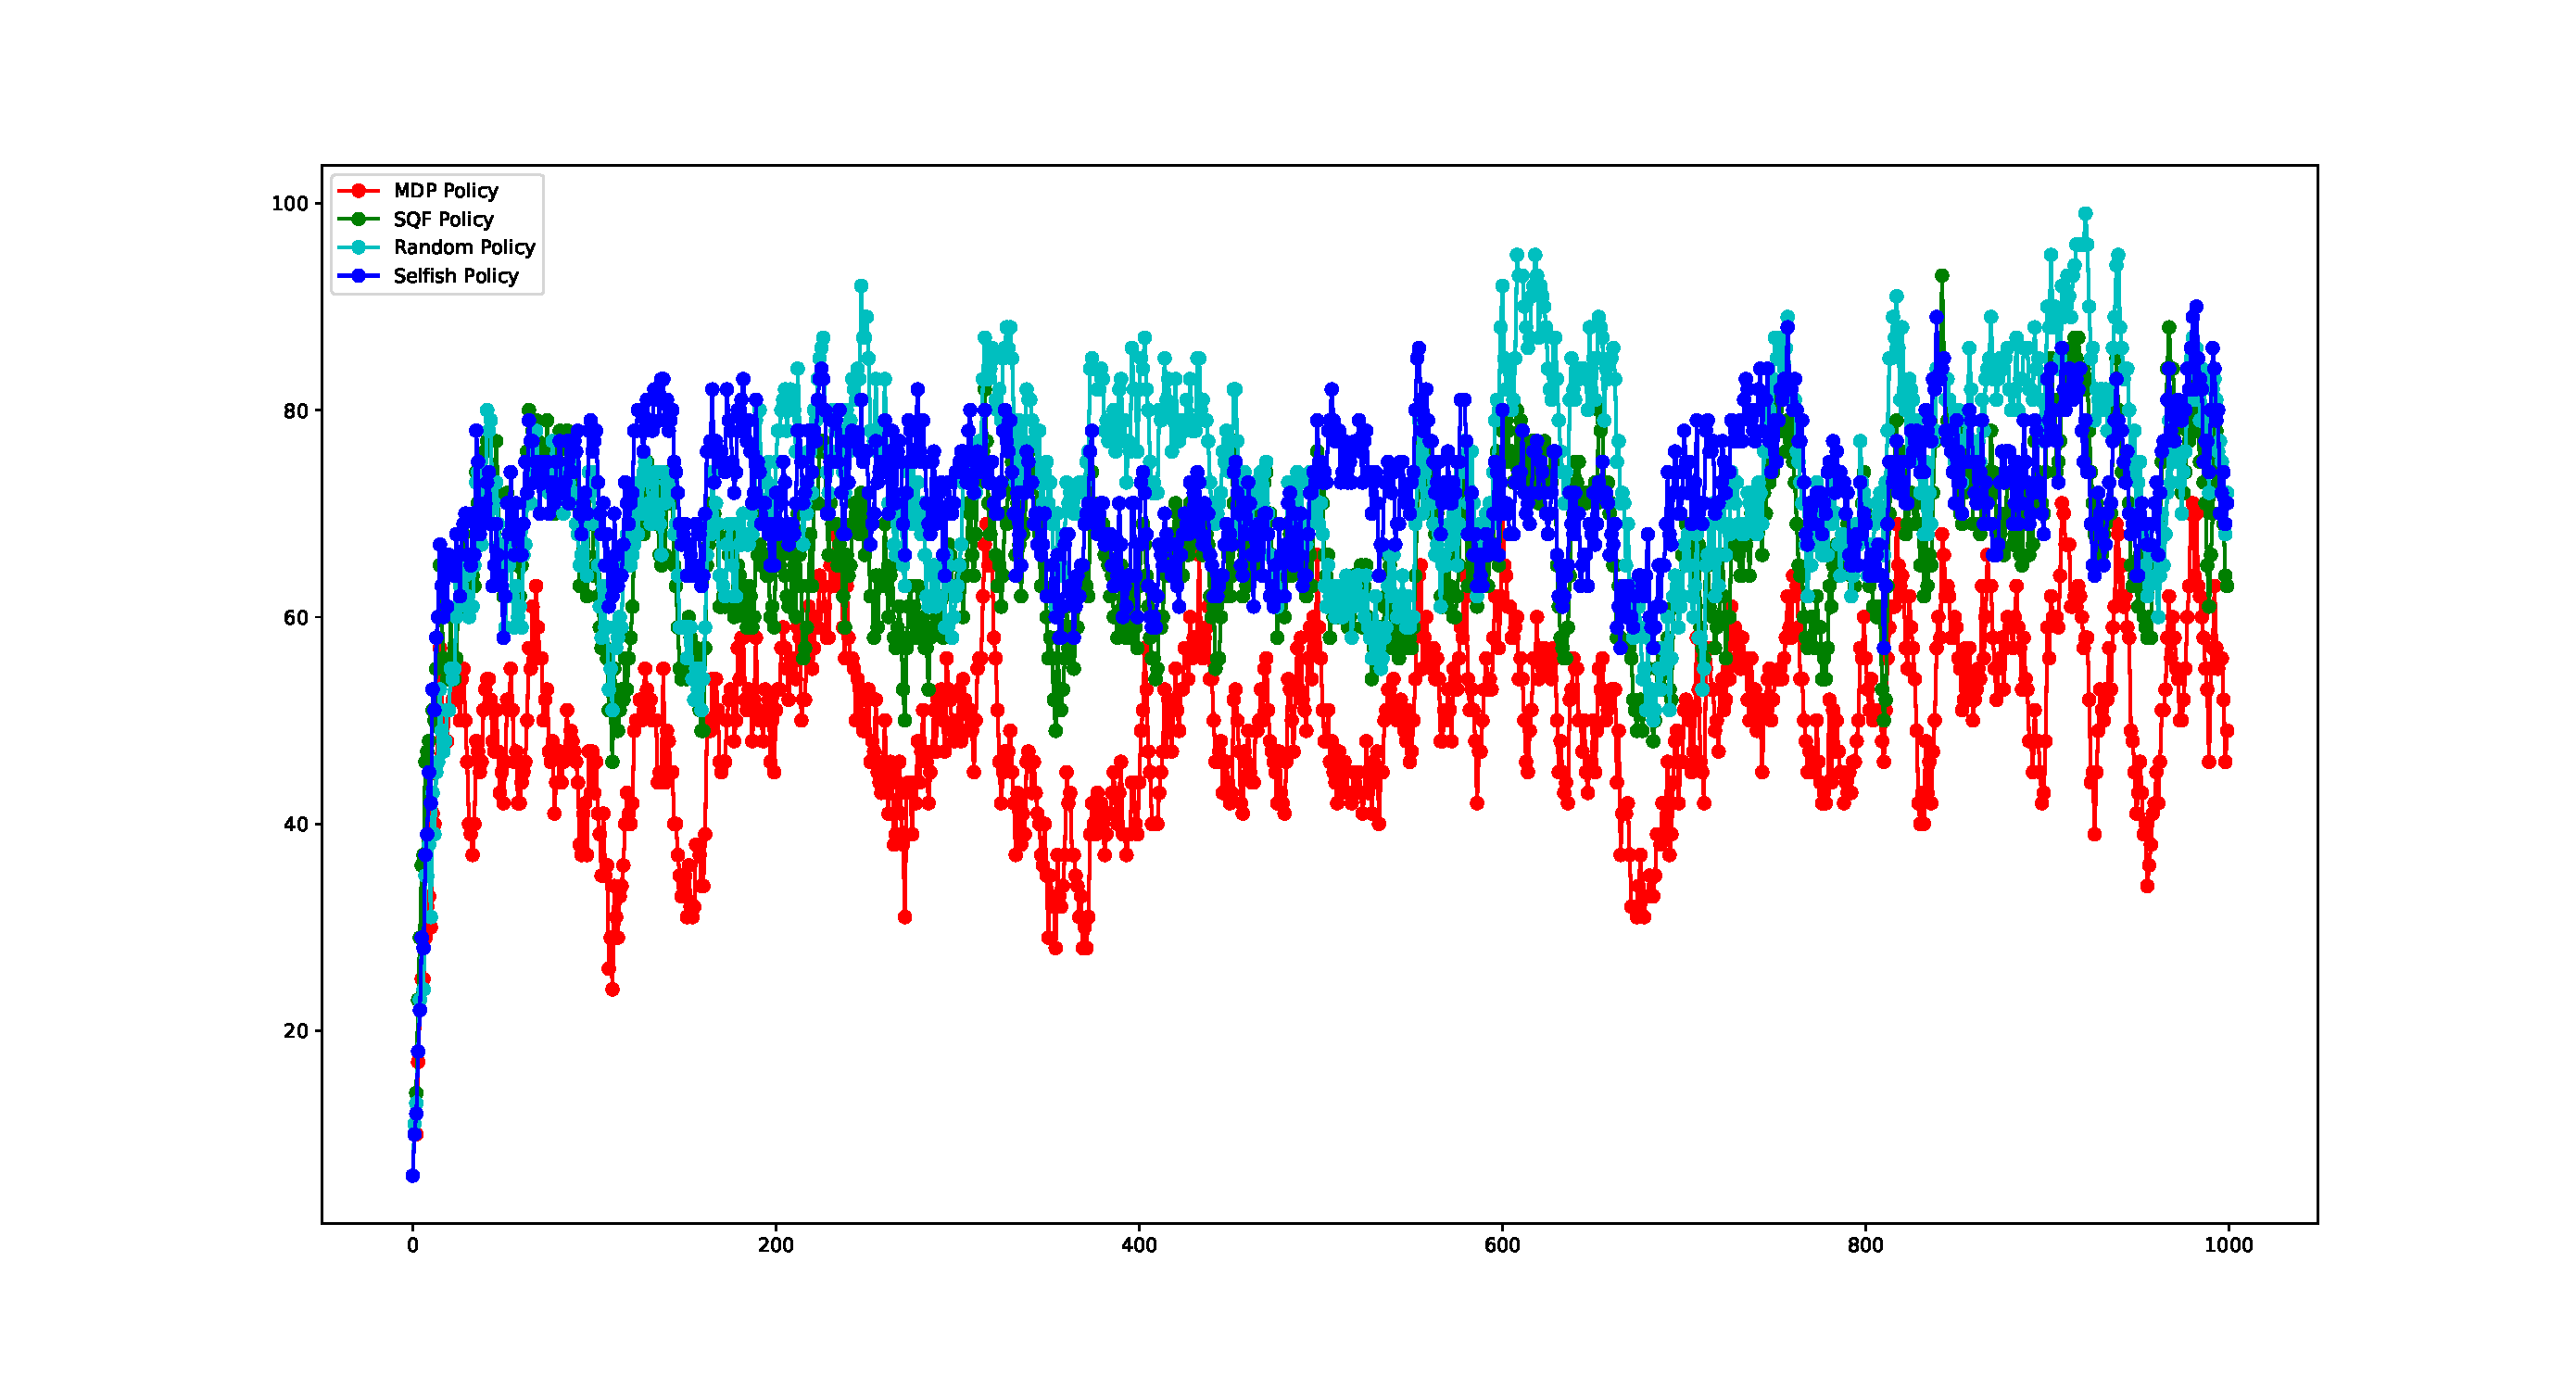
\includegraphics[width=0.80\textwidth]{images/Figure_1.pdf}
    \caption{Timeline illustration.}
    \label{fig:general_timeline}
\end{figure*}

\textbf{Compared Algorithms:}
We compare the proposed algorithm with other three heuristic algorithms which are listed as follows.
\begin{itemize}
    \item \textbf{Random Dispatching Policy}:
            for each job type, randomly choose the dispatching edge server in each time slot; 
    \item \textbf{Selfish Algorithm}:
            for each job type, always choose the edge server with the minimum expected uploading time, plus the expected processing time;
    \item \textbf{Queue-aware Selfish Algorithm}:
            for each job type, always choose the edge server with the minimum expected uploading time, plus the expected processing time and queueing time based on the observation of outdated queue states.
\end{itemize}
Specifically, we choose the \emph{Local Selfish Algorithm} which is state-invariant as the initial fixed policy for our proposed algorithm.
The explicit definition is given as follows.
\begin{policy}[Selfish Policy]
    \begin{align}
        \Baseline &\define \Brace{ \Pi_{k}\define\set{\pi_{k,j}|\forall j\in\jSpace} |\forall k\in\apSet },
        \\
        \pi_{k,j} &\define \arg\min_{m\in\esSet_{k}} u_{k,m,j} + c_{m,j}
    \end{align} 
\end{policy}
%----------------------------------------------------------------------------------------%

\subsection{Performance Analysis}
    \subsubsection{Basic Performance}
    Here we measure some basic metrics concerning in edge computing system, compared with different algorithms.
    \begin{itemize}
        \item Bar graph: Average Cost v.s. Algorithms, Fig.\ref{fig:bar_plot}(a);
        \item Bar graph: Average JCT (job completion time) v.s. Algorithms, Fig.\ref{fig:bar_plot}(b); %also shows sampling is uniform and acceptable (between chosen average cost and actual average JCT)
        \item Bar graph: Average Departure Rate (throughput) v.s. Algorithms, Fig.\ref{fig:bar_plot}(c). 
    \end{itemize}

    \subsubsection{Fine-grained Analysis}
    \begin{itemize}
        \item \fixit{Timeline graph: our proposed algorithm is better than compared algorithms all the time};
        \item CDF graph of Cost (with different algorithms);
        \item CDF graph of JCT (with different algorithms);
    \end{itemize}

    \begin{figure}[h]
        \centering
        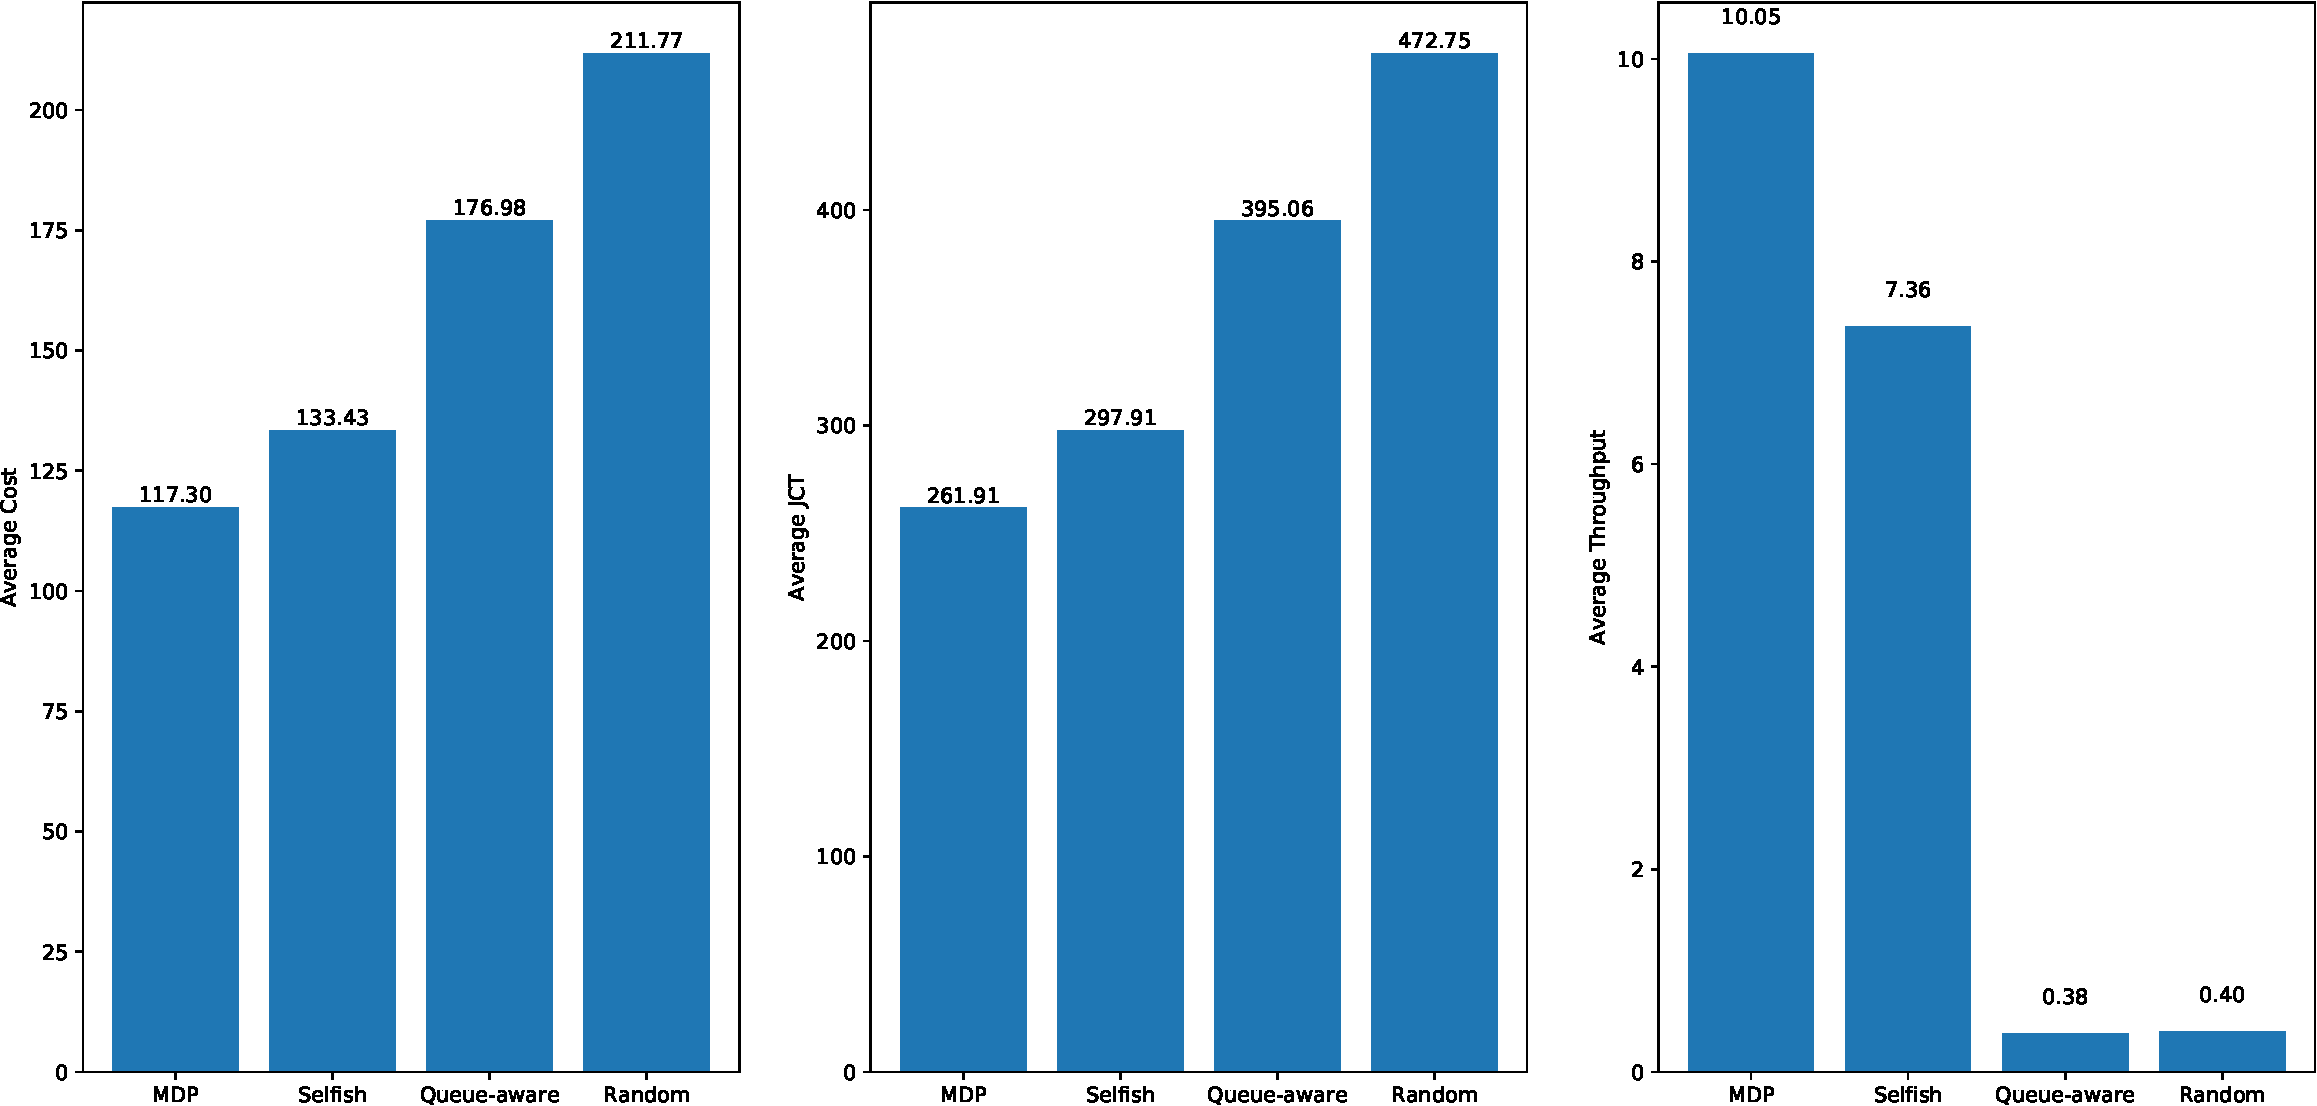
\includegraphics[width=0.45\textwidth]{images/bar_graph.pdf}
        \caption{Basic performance comparison.}
        \label{fig:bar_plot}
    \end{figure}

    \subsubsection{Sensitivity Study}
    \begin{itemize}
        \item \textbf{Compared with different \brlatency.} Fig.\ref{fig:eval_delay}
        \item \textbf{Different number of APs.} (a.k.a arrival rate)
        \item \textbf{Different $t_B$ setting.}
        \item \textbf{Uploading time domains/Processing time domains.}
        % \item \textbf{Different Penalty Factors.}
    \end{itemize}
    % CDF of \# of dropped jobs (over the queue limit); CDF of queue length;

    \begin{figure*}[ht!]
        \centering
        \begin{tabular}{ccc}
            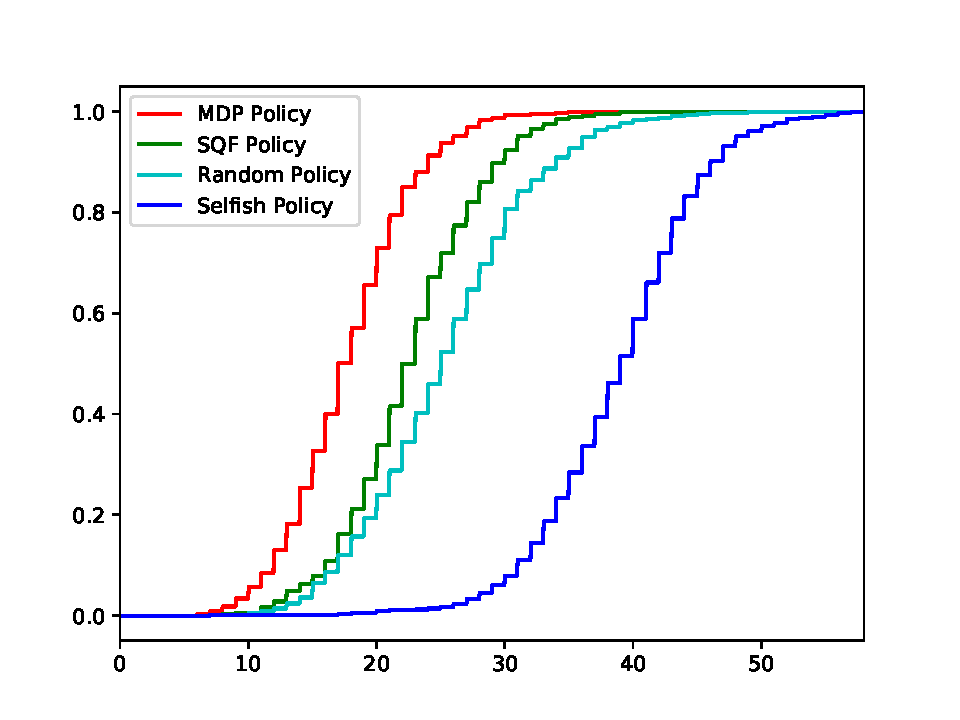
\includegraphics[width=0.30\textwidth]{images/535_LowPressure_NoDelay.pdf}&
            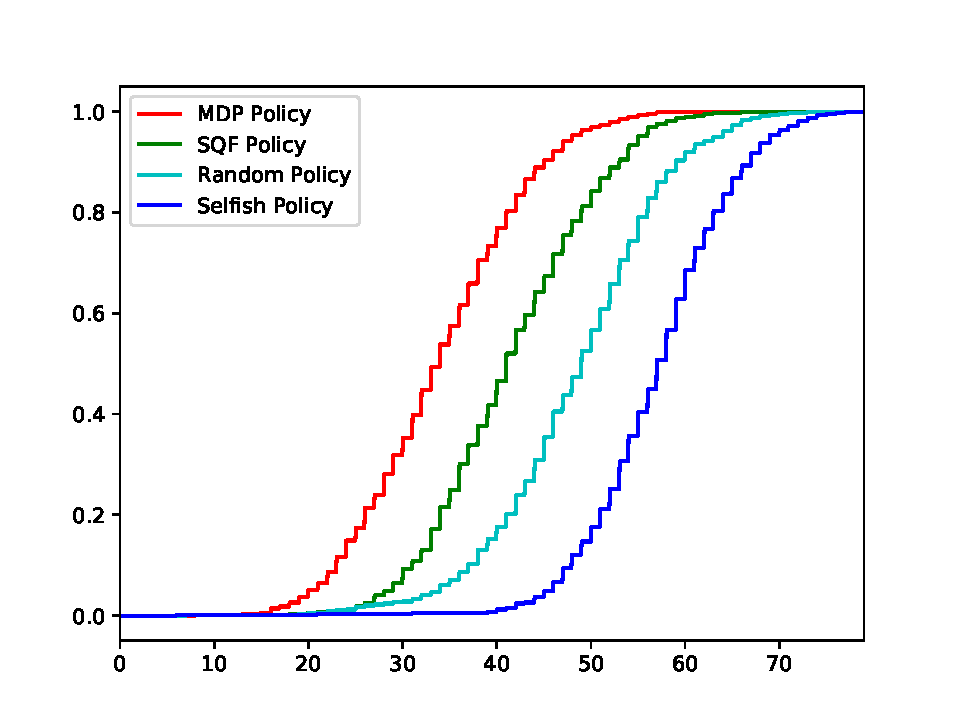
\includegraphics[width=0.30\textwidth]{images/535_LowPressure_LargeDelay_cdf.pdf}&
            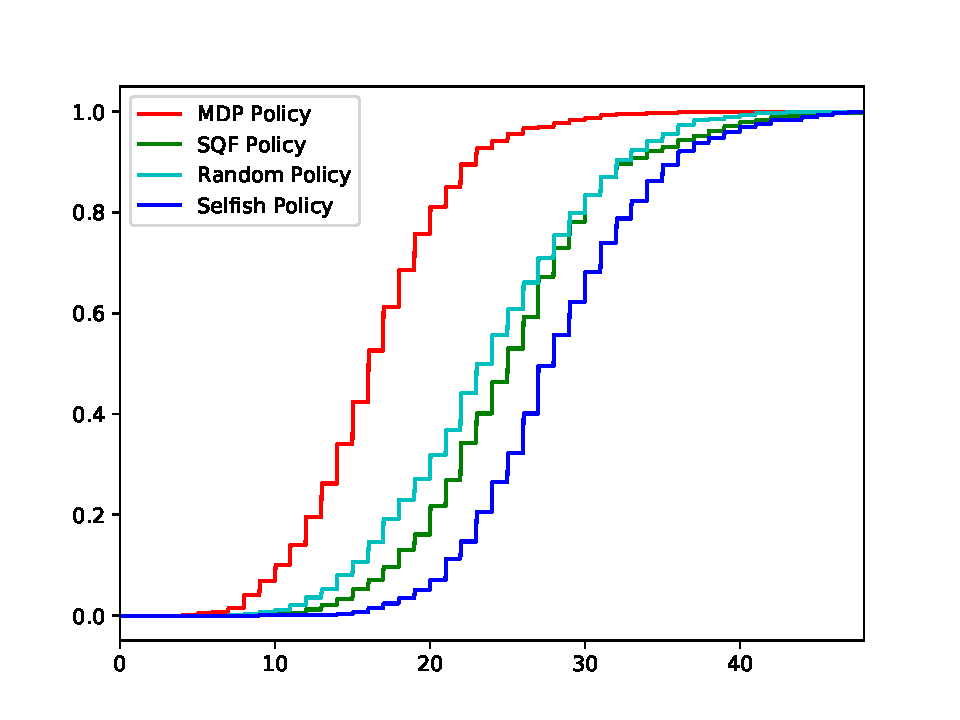
\includegraphics[width=0.30\textwidth]{images/535_LowPressure_FullDelay.pdf}
            \\
            {\small (a) No \brlatency} &
            {\small (b) Large \brlatency} &
            {\small (c) Whole-interval \brlatency}
        \end{tabular}
        \caption{Evaluation of Information Staleness Impact on Algorithm Robustness under Low Back Pressure.}
        \label{fig:eval_delay}
    \end{figure*}

    % \begin{figure}[h]
    %     \centering
    %     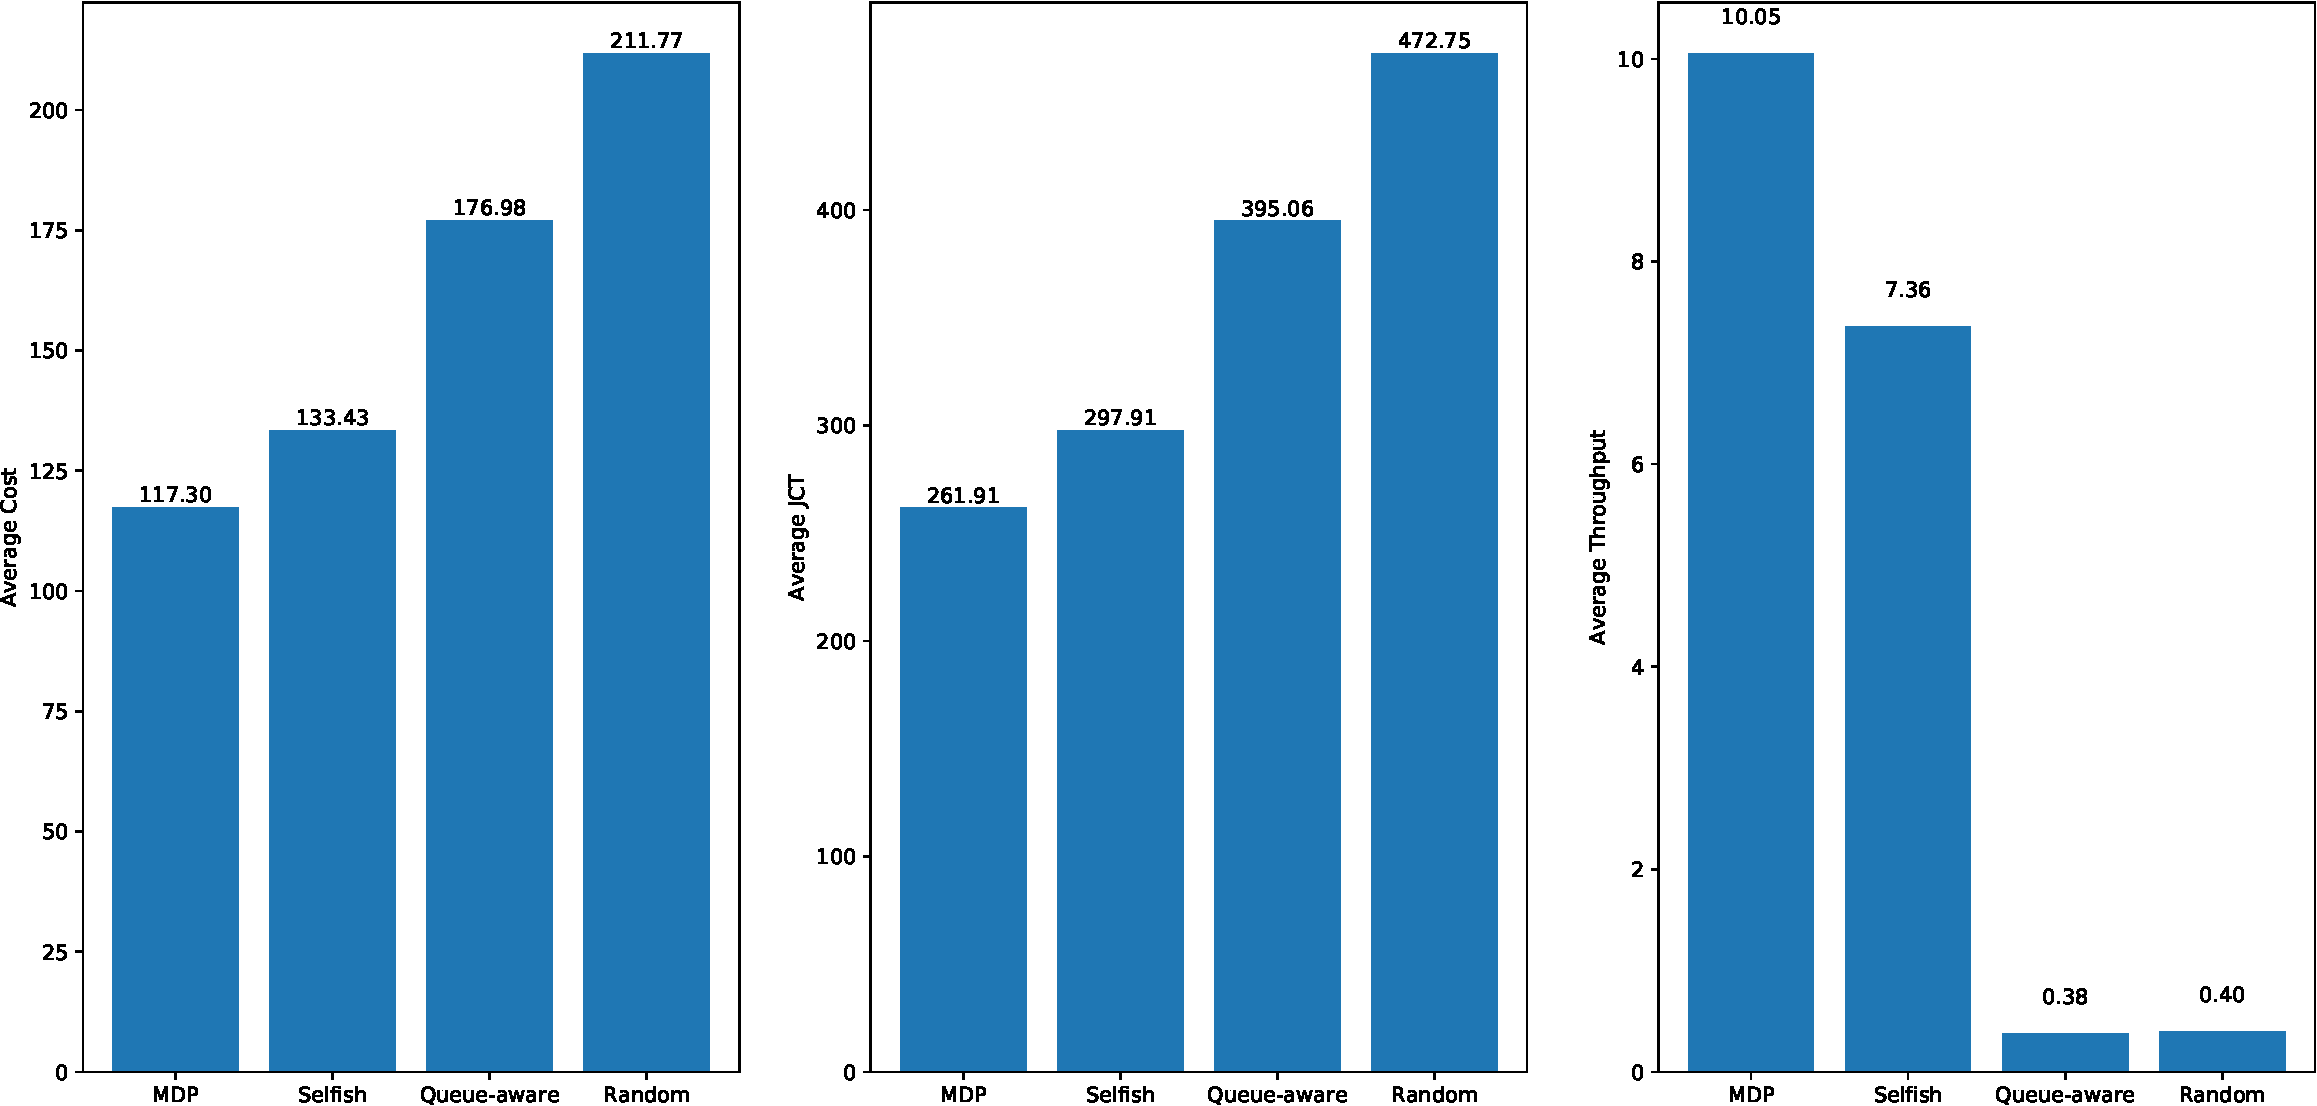
\includegraphics[width=0.45\textwidth]{images/bar_graph.pdf}
    %     \caption{Fake.}
    %     \label{fig:bar_plot}
    % \end{figure}
    % \begin{figure}[h]
    %     \centering
    %     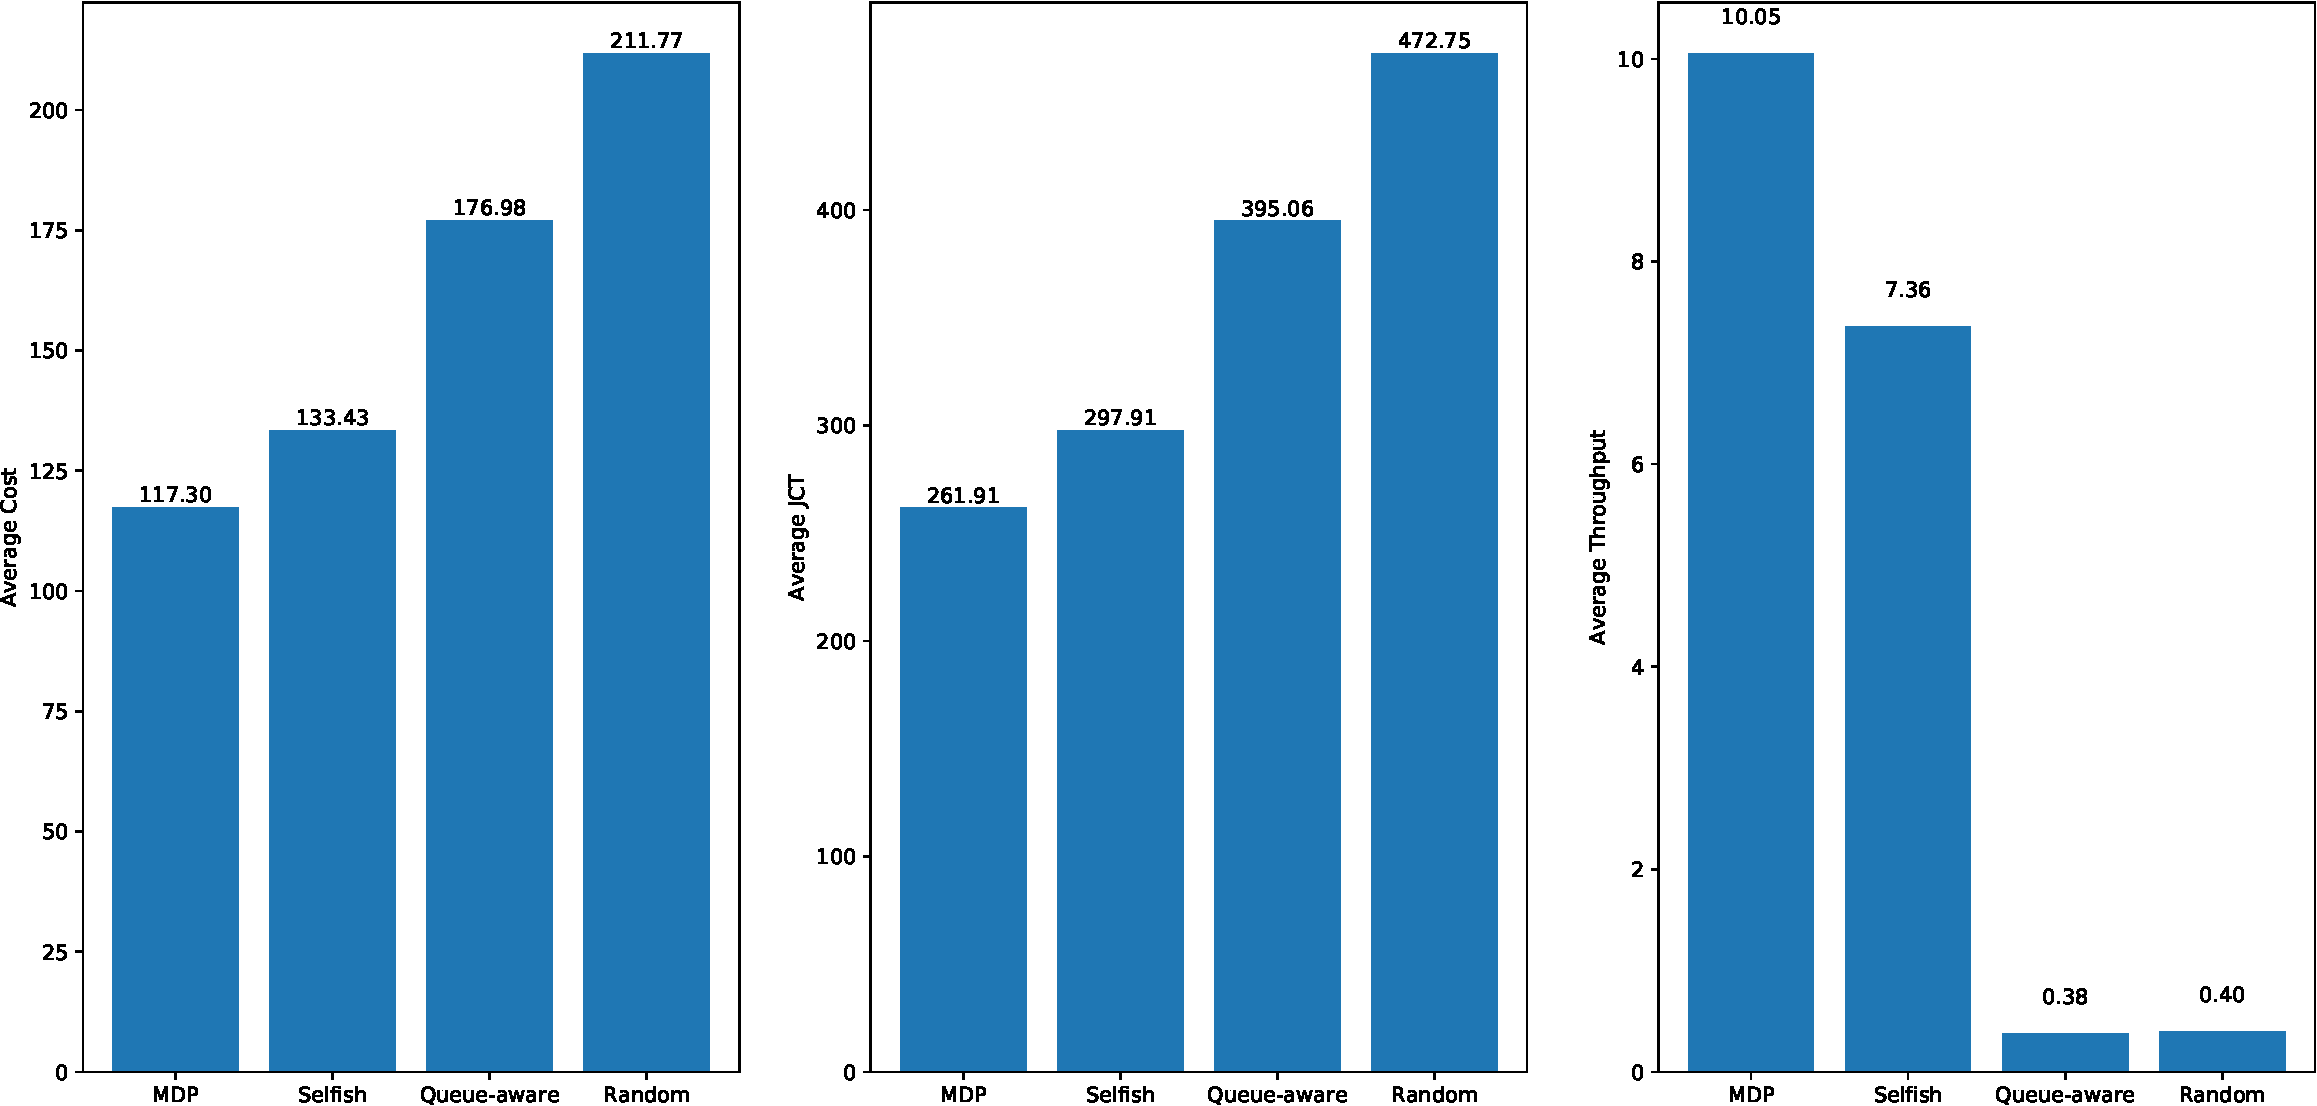
\includegraphics[width=0.45\textwidth]{images/bar_graph.pdf}
    %     \caption{Fake.}
    %     \label{fig:bar_plot}
    % \end{figure}
    % \begin{figure}[h]
    %     \centering
    %     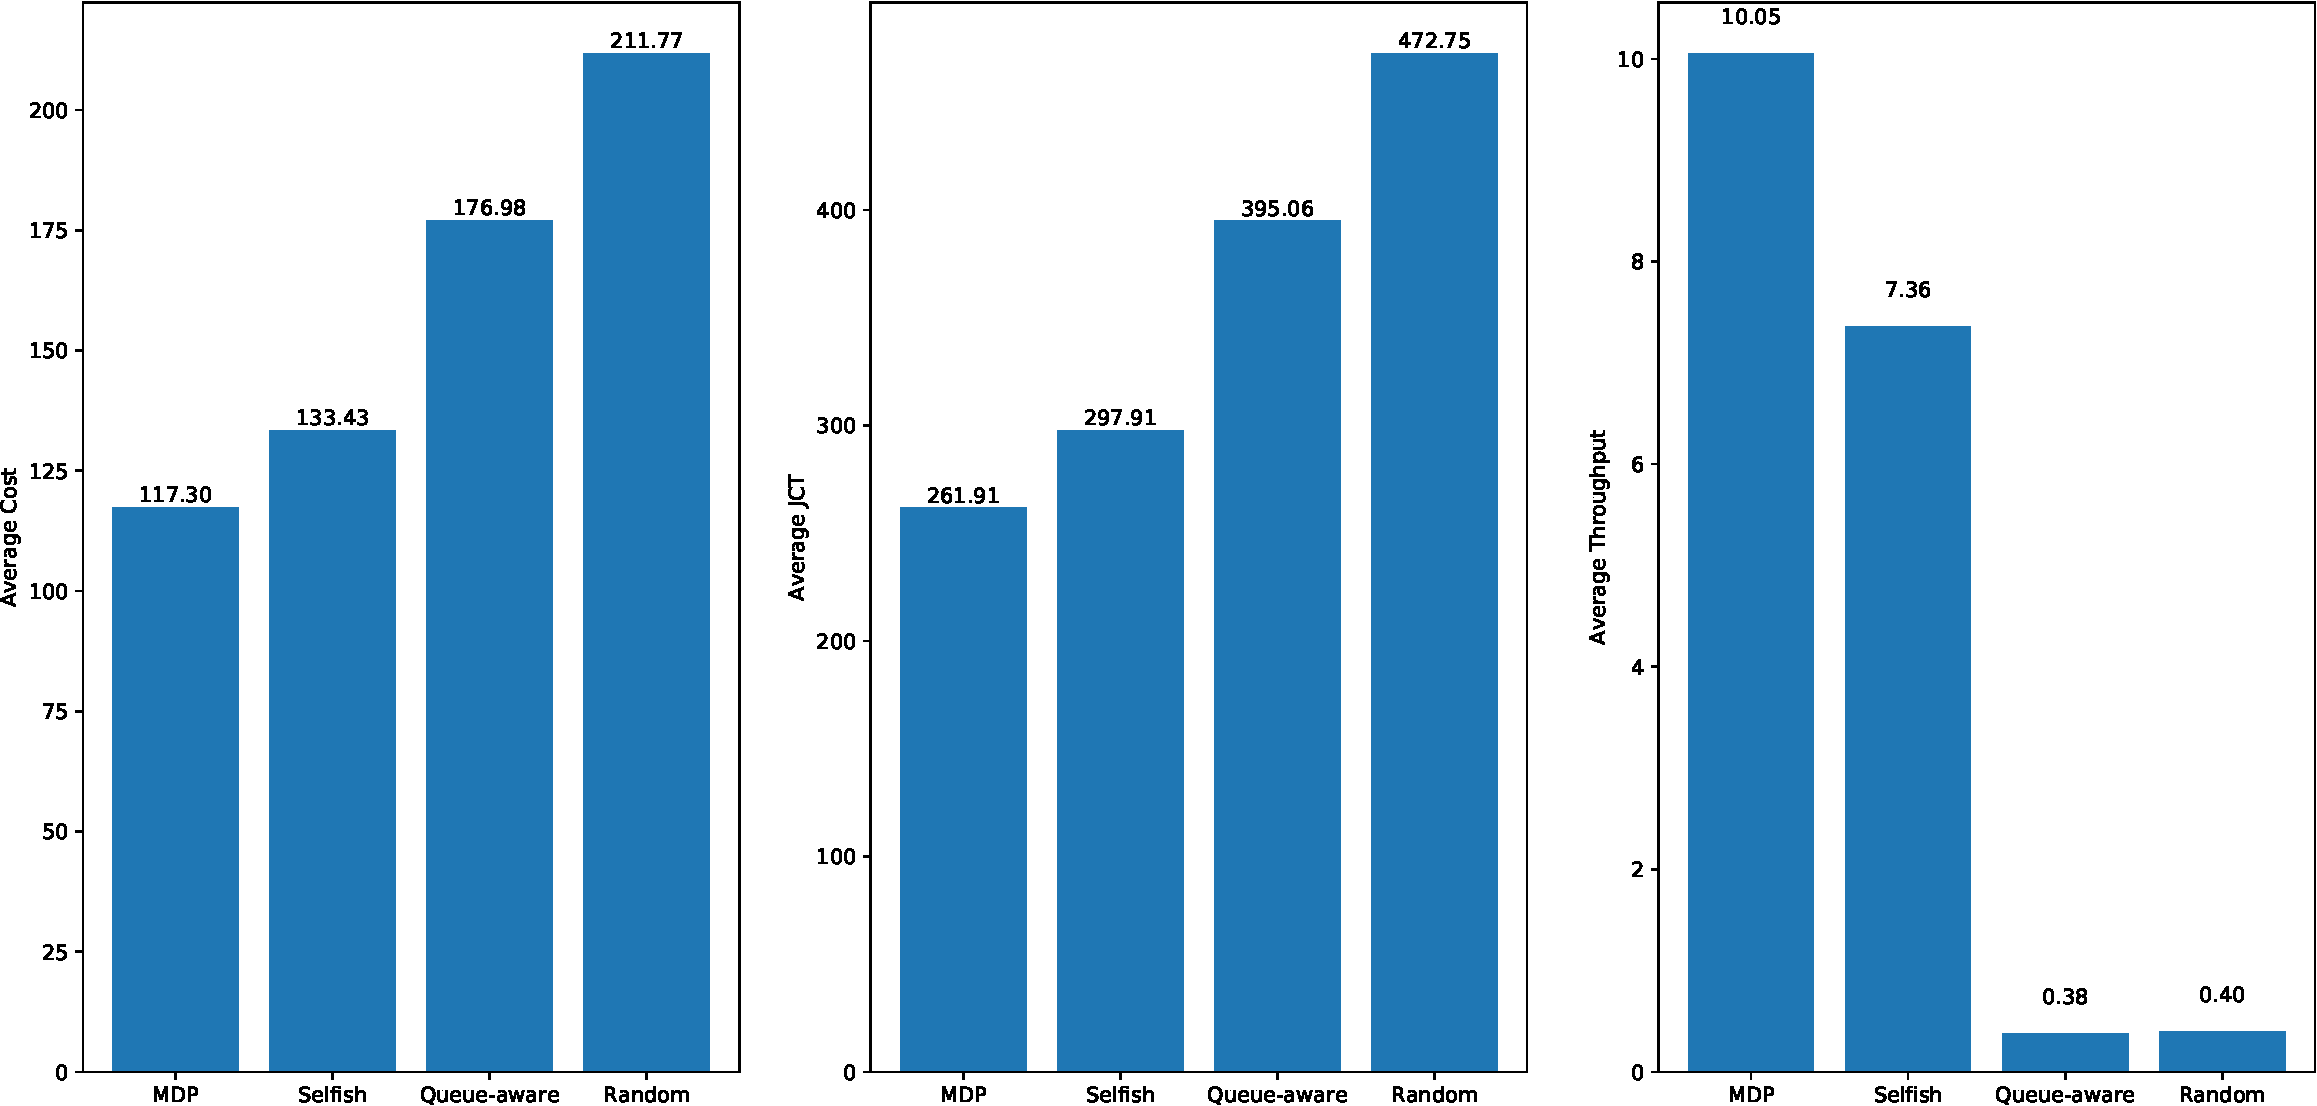
\includegraphics[width=0.45\textwidth]{images/bar_graph.pdf}
    %     \caption{Fake.}
    %     \label{fig:bar_plot}
    % \end{figure}
    % \begin{figure}[h]
    %     \centering
    %     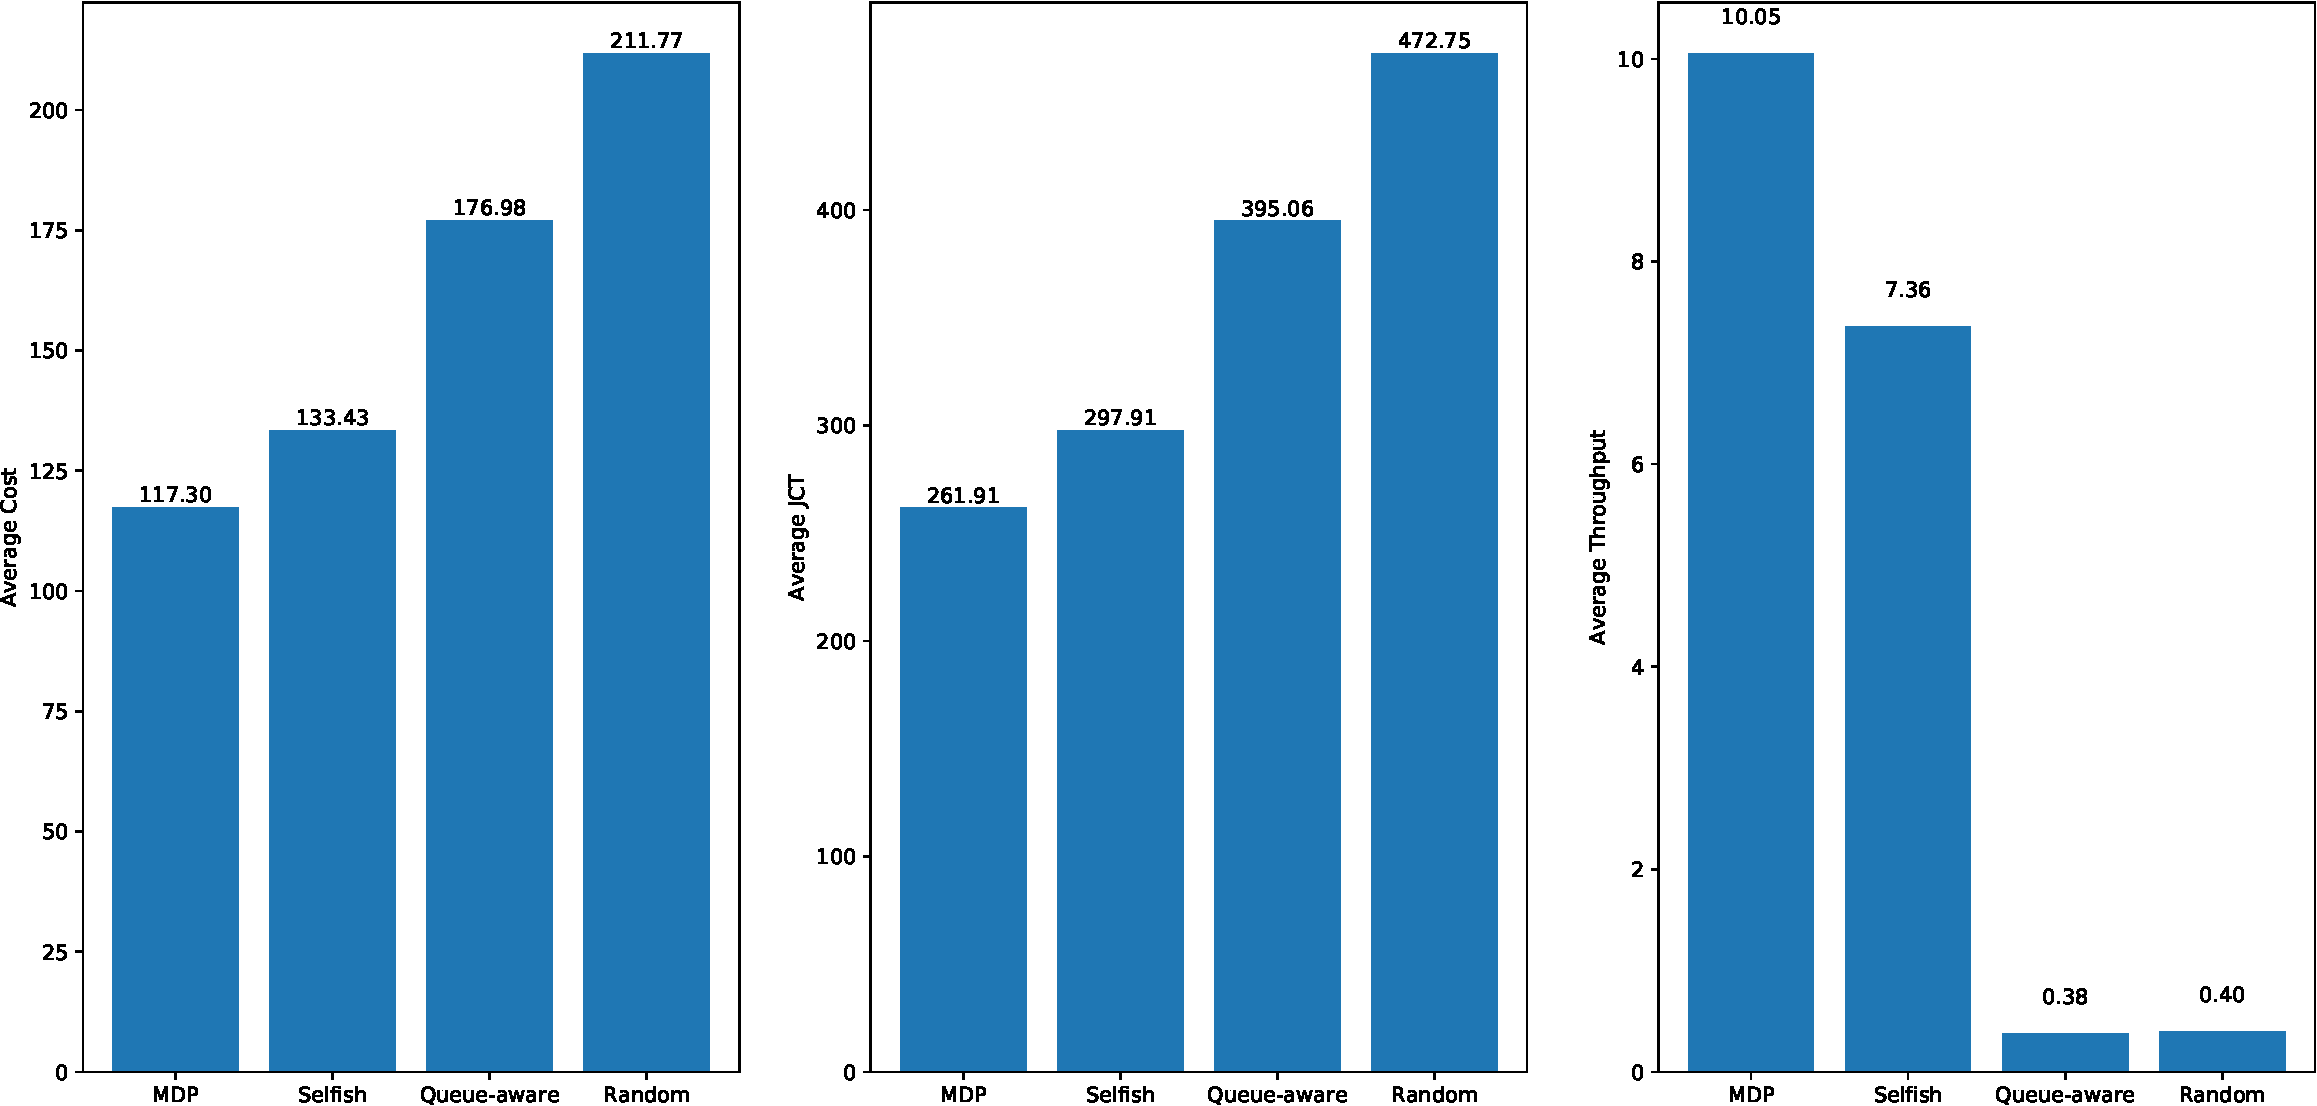
\includegraphics[width=0.45\textwidth]{images/bar_graph.pdf}
    %     \caption{Fake.}
    %     \label{fig:bar_plot}
    % \end{figure}
%----------------------------------------------------------------------------------------%

\delete{v19}{
    \textbf{Data Trace Extraction:}
    We use the Google data trace for cloud computing\needref{google-data-trace}.
    There is no broadcast latency, uploading time, and processing distribution information specified in the data trace.
    Hence, we extract and scale the arrival and processing time in the original data trace.
    And we manipulate the original data with random generated latency distribution.

    % [abandon, cause useless]
    \textbf{Estimation Error Analysis.}
    (If these graphs are not good, they are not going to appear on final draft.)
    \begin{itemize}
        \item Two curves, one for real cost against time slot, one for expected sampling cost against time intervals; (if the accumulate area within the latter one has little/bounded error with real cost, then it is okay and the correctness is support by simulation) 
    \end{itemize}
}